
\chapter{Serverless Architecture}
\authors{Ryan Christensen Wang, Steven Tanaka, Yogi Valentino Nadeak}

	\gny{Tolong tambahkan keterangan gambar contoh : Gambar 8.1, 8.2, dst.. dan tambahkan italic text untuk setiap bahasa asing}
	
\section{Definisi Serverless Architechture}
Serverless architecture merupakan pendekatan dalam desain software yang mana developer tidak perlu pusing-pusing lagi mengelola infrastruktur seperti server.Developer bisa fokus dalam mengembangkan aplikasinya dan masalah server akan dikelola oleh penyedia layanan serverless (provider).

Less dalam serverless bukan berarti tanpa server sama sekali, tetapi memungkinkan untuk konfigurasi seminimal mungkin atau dikurangi. Misalnya, pengembang tidak perlu tidak perlu otak-atik konfigurasi web server ketika melakukan deploy kode yang hanya tinggal dihubungkan ke proxy.

Developer menggunakan Serverless Architecture untuk menggunakan kembali layanan dalam sistem yang berbeda atau menggabungkan beberapa layanan independen untuk melakukan tugas yang kompleks. 

Misalnya, beberapa proses bisnis dalam suatu organisasi memerlukan fungsionalitas autentikasi pengguna. Alih-alih menulis ulang kode autentikasi untuk semua proses bisnis, Anda dapat membuat satu layanan autentikasi dan menggunakannya kembali untuk semua aplikasi. Demikian juga dengan sistem di seluruh organisasi layanan kesehatan, seperti sistem manajemen pasien dan sistem catatan kesehatan elektronik (EHR), sebagian besar perlu mendaftarkan pasien. Sistem ini dapat memanggil satu layanan umum untuk melakukan tugas pendaftaran pasien.

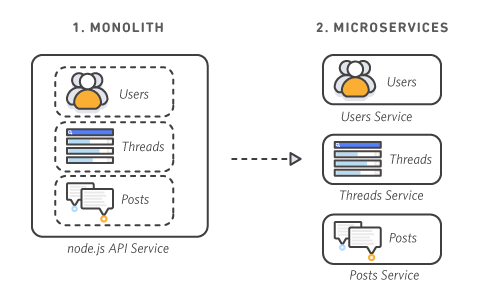
\includegraphics[width=\textwidth]{Mono.png}

\textbf{Ada beberapa istilah dasar dalam arsitektur ini, antara lain:}

\begin{itemize}
	\item \textbf{Invocation,} yaitu eksekusi fungsi tunggal.
	\item \textbf{Duration,} durasi waktu yang dibutuhkan fungsi serverless
	\item \textbf{Cold start,} yaitu terjadinya latensi saat fungsi ter-trigger pertama kali atau setelah periode tidak aktif.
	\item \textbf{Concurrency limit,} yaitu jumlah fungsi instance yang dapat dijalankan secara bersamaan dalam satu wilayah
	\item \textbf{Timeout,} yaitu jumlah waktu yang diizinkan oleh penyedia layanan untuk menjalankan fungsi sebelum dihentikan.
\end{itemize}

Serverless architecture ini cocok digunakan untuk kasus yang melakukan tugas jangka pendek dan mengelola beban kerja yang mengalami lalu lintas yang jarang dan tidak dapat diprediksi. Ada beberapa kasus lain yang dapat dipertimbangkan menggunakan arsitektur ini, yaitu:

\begin{itemize}
	\item Tugas yang berdasarkan trigger
	\item Membangun RESTful API
	\item Continuous Integration dan Continuous Delivery (CI/CD)
	\item Proses asinkronus
\end{itemize}

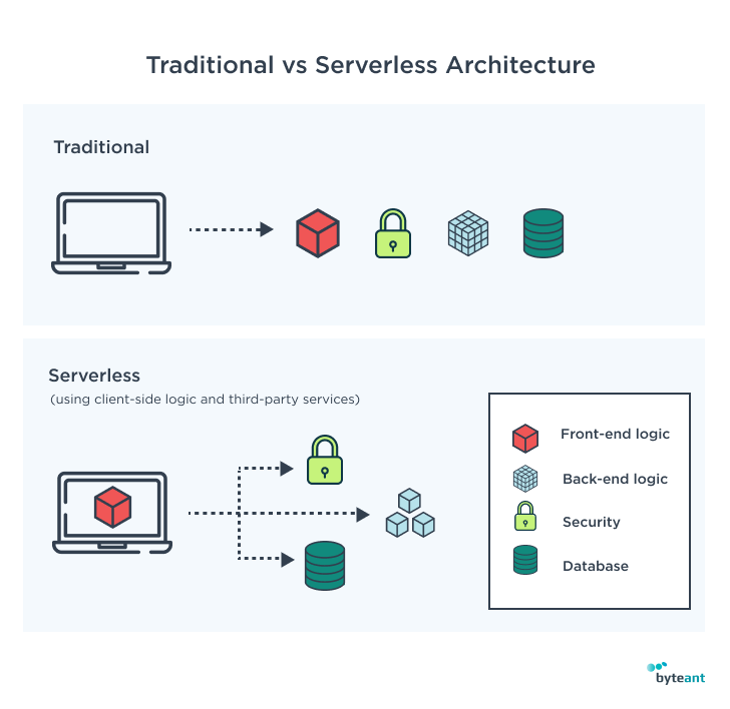
\includegraphics[width=\textwidth]{Archi.png}

\section{Fungsi/Kegunaan dari Serverless Architecture}

Serverless architecture adalah sebuah model komputasi di awan yang mana penyedia layanan awan bertanggung jawab dalam mengelola infrastruktur dan memperuntukan sumber daya komputasi yang dibutuhkan secara otomatis, tanpa pengguna perlu mengurus atau merawat server. Terdapat beberapa keuntungan dari penggunaan arsitektur serverless, diantaranya adalah:

Penilaian untuk setiap karakteristik berdasarkan kecenderungan alami untuk implementasi tipikal pola layered.

\begin{itemize}
	\item optimisasi biaya dengan hanya membayar untuk sumber daya yang digunakan
	\item memungkinkan pengembangan aplikasi yang lebih cepat
	\item skalabilitas yang mudah untuk mengakomodasi perubahan permintaan
	\item serta perawatan dan pemeliharaan yang lebih mudah karena dikelola oleh penyedia layanan awan.
\end{itemize}

\section{Kekurangan dan Kelebihan dari Serverless Architecture}
\subsection{Kelebihan dari Serverless Architecture}

\begin{itemize}
	\item \textbf{Skalabilitas:} Dalam arsitektur serverless, aplikasi dapat dengan mudah ditingkatkan kapasitasnya untuk menangani permintaan yang berfluktuasi, sehingga dapat mengurangi pengeluaran untuk infrastruktur yang tidak terpakai.
	\item \textbf{Biaya operasional yang rendah:} Dalam serverless, pengguna hanya membayar untuk sumber daya yang mereka gunakan, yang dapat mengurangi biaya operasional secara signifikan.
	\item \textbf{Fokus pada pengembangan aplikasi:} Dalam serverless, pengembang tidak perlu khawatir mengurus infrastruktur server dan dapat fokus pada pengembangan aplikasi.
	\item \textbf{Perawatan dan pemeliharaan yang mudah:} Dalam serverless, penyedia layanan awan bertanggung jawab atas perawatan dan pemeliharaan infrastruktur, sehingga pengguna tidak perlu memikirkan pembaruan sistem operasi atau patch keamanan.
\end{itemize}

\subsection{Kekurangan dari Serverless Architecture}

\begin{itemize}
	\item \textbf{Keterbatasan dalam penggunaan:} Serverless mungkin tidak cocok untuk semua jenis aplikasi, terutama jika aplikasi memerlukan kontrol tinggi atas infrastruktur dan lingkungan di mana aplikasi berjalan.
	\item \textbf{Ketergantungan pada penyedia layanan awan:} Serverless membuat pengguna sangat bergantung pada penyedia layanan awan, sehingga jika terjadi masalah atau gangguan pada layanan, aplikasi dapat mengalami downtime yang signifikan.
	\item \textbf{Pengaturan konfigurasi yang kompleks:} Serverless dapat memiliki konfigurasi yang kompleks dan memerlukan pengaturan yang cermat untuk memastikan aplikasi berjalan dengan baik.
	\item \textbf{Performa yang tidak stabil:} : Serverless dapat mengalami performa yang tidak stabil jika pengguna tidak melakukan penyesuaian yang cermat dalam skala dan konfigurasi aplikasi.
\end{itemize}

\section{Penerapan Serverless Architecture}
	Serverless Architecture adalah model komputasi awan di mana penyedia awan secara dinamis mengelola alokasi dan penyediaan server, memungkinkan pengembang untuk fokus menulis kode tanpa harus mengelola infrastruktur.
	
	Berikut adalah beberapa contoh penerapan serverless architecture:
	\begin{itemize}
		\item \textbf{Web applications:} Pengembang dapat membangun dan menerapkan aplikasi web menggunakan arsitektur tanpa server, tanpa harus mengelola server atau infrastruktur. Mereka dapat menggunakan layanan seperti AWS Lambda, Google Cloud Functions, atau Azure Functions untuk menulis kode yang merespons kejadian, seperti permintaan HTTP, dan berjalan sesuai permintaan.
		\item \textbf{Data processing:} Serverless Architecture dapat digunakan untuk tugas pemrosesan data seperti transformasi data, pembersihan, dan analisis. Pengembang dapat menggunakan layanan seperti AWS Glue, Google Cloud Dataflow, atau Azure Stream Analytics untuk memproses data tanpa server, tanpa harus mengelola server atau infrastruktur.
		\item \textbf{Chatbots:} Pengembang dapat membangun chatbot menggunakan serverless, dengan menulis kode yang merespons acara obrolan, seperti pesan pengguna. Mereka dapat menggunakan layanan seperti AWS Lex, Google Cloud Dialogflow, atau Azure Bot Service untuk membuat dan menerapkan chatbot yang berjalan sesuai permintaan.
		\item \textbf {IoT applications:} Serverless Architecture dapat digunakan untuk aplikasi IoT, dengan memungkinkan pengembang menulis kode yang merespons kejadian dari perangkat IoT, seperti pembacaan sensor. Mereka dapat menggunakan layanan seperti AWS IoT, Google Cloud IoT Core, atau Azure IoT Hub untuk membangun dan menerapkan aplikasi IoT tanpa server.
	\end{itemize}


